\begin{frame}{Regression Example}
    The \texttt{faithful} dataset in \texttt{R} has two measurements taken for the Old Faithful Geyser in Yellowstone National Park:
    \begin{itemize}
        \item \texttt{eruptions}: the length of each eruption
        \item \texttt{waiting}: the time between eruptions
    \end{itemize}
    Each is measured in minutes.
\end{frame}

\begin{frame}{Regression Example}
    We want to see if we can use the wait time to \textit{predict} eruption duration.
    \begin{itemize}
        \item \texttt{eruptions} will be the response variable.
        \item \texttt{waiting} will be the predictor variable.
    \end{itemize}
\end{frame}

\begin{frame}{Regression Example}
    \begin{center}
        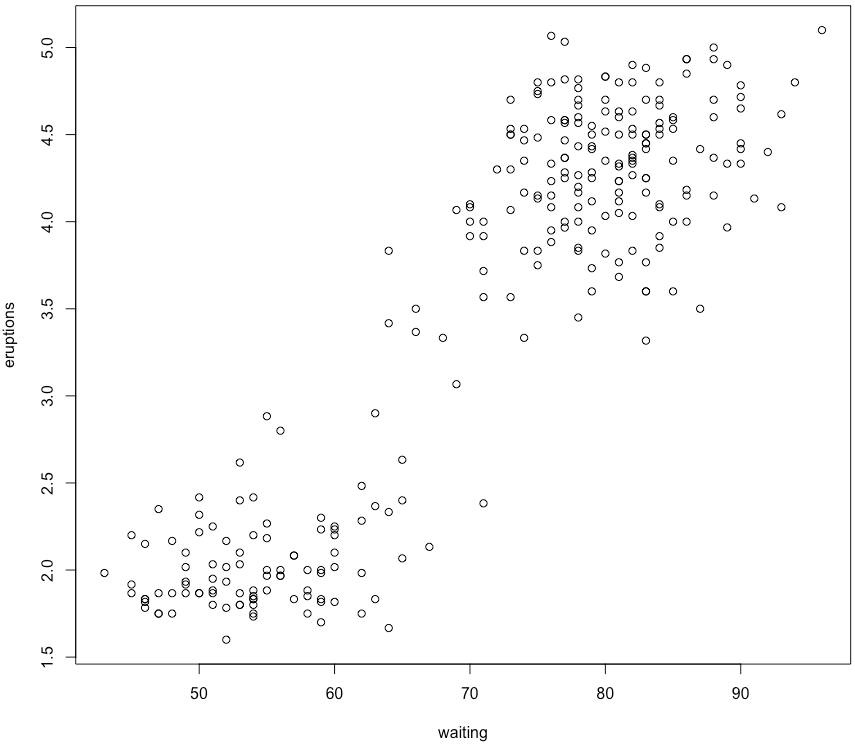
\includegraphics[scale=0.25]{images/geyserscatter.png}
    \end{center}
\end{frame}

\begin{frame}{Regression Example}
    Using \texttt{R}, the estimated regression line for
    \[
        \texttt{eruptions} = \beta_0 + \beta_1 \texttt{waiting} + \epsilon
    \]
    is found to be
    \[
        \hat{y} = -1.8740 + 0.0756 x
    \]
\end{frame}

\begin{frame}{Regression Example}
    \begin{center}
        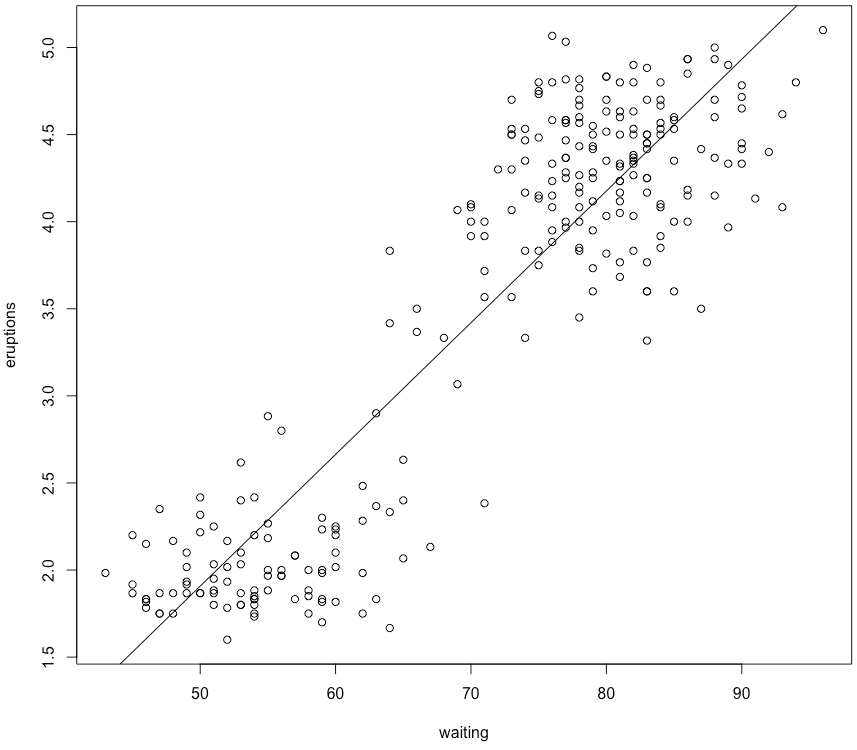
\includegraphics[scale=0.25]{images/geysreg.png}
    \end{center}
\end{frame}

\begin{frame}{Regression Example}
    \begin{itemize}
        \item In this data, waiting times range from 43 minutes to 96 minutes. 
        \item Let's predict
        \begin{itemize}
            \item eruption time for a 50 minute wait.
            \item eruption time for a 10 minute wait.
        \end{itemize}
    \end{itemize}
\end{frame}

\begin{frame}{Regression Example}
    For $\texttt{waiting}=x=50$,
    \begin{align*}
        \hat{y} &= -1.8740 + 0.0756 x \\
        &= -1.8740 + 0.0756 \times 50 \\
        &= 1.906
    \end{align*}
    So for a wait time of 50 minutes, the predicted average eruption time is 1.906 minutes.
\end{frame}

\begin{frame}{Regression Example}
    For $\texttt{waiting}=x=10$,
    \begin{align*}
        \hat{y} &= -1.8740 + 0.0756 x \\
        &= -1.8740 + 0.0756 \times 10 \\
        &= -1.118
    \end{align*}
    So for a wait time of 10 minutes, the predicted average eruption time is -1.118 minutes.
\end{frame}

\begin{frame}{Regression Example}
    But a predicted average eruption time of -1.118 minutes
    \begin{enumerate}
        \item doesn't make sense.
        \item is an extrapolation!
    \end{enumerate}
    We do not want to make this prediction.
\end{frame}

\begin{frame}{Regression Example}
    \vspace{-18pt}\begin{center}
        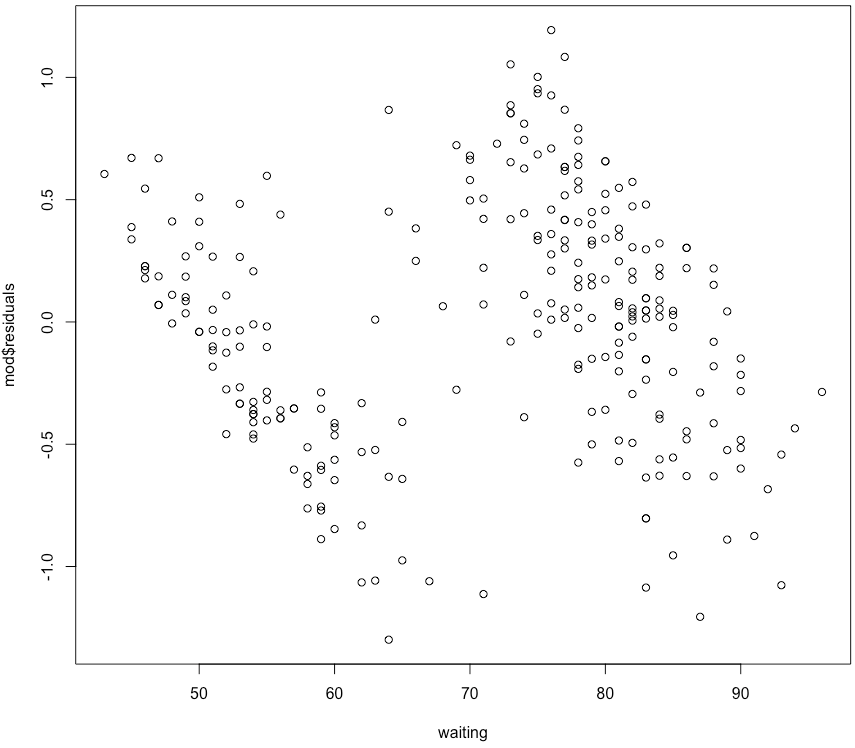
\includegraphics[scale=0.25]{images/geyserResid.png}
    \end{center}
    \vspace{-12pt}This is the residual plot for the geyser regression. Do you see any problems?
\end{frame}

\begin{frame}{Regression Example}
    \vspace{-18pt}\begin{center}
        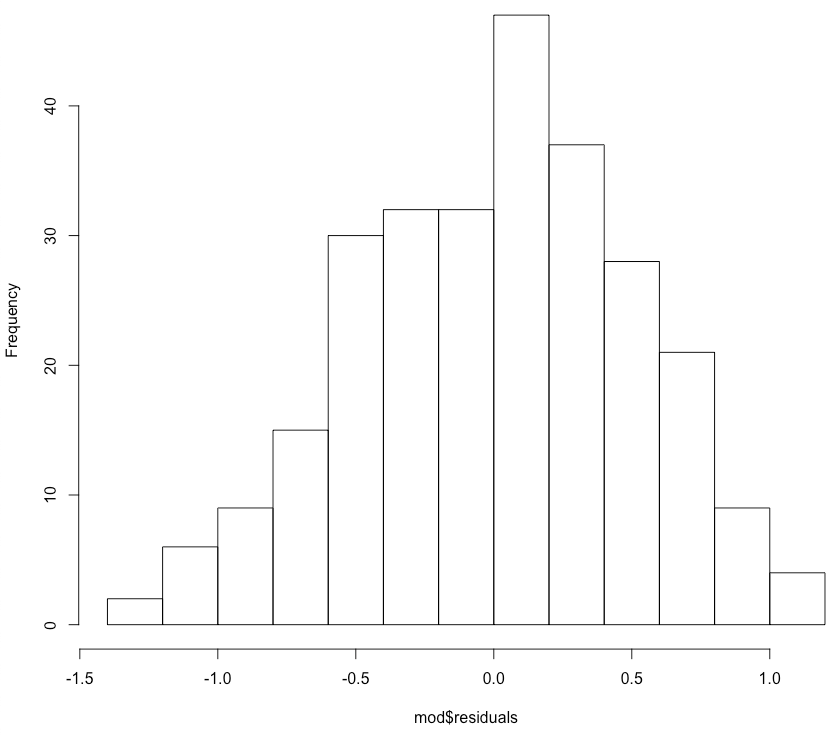
\includegraphics[scale=0.25]{images/residhist.png}
    \end{center}
    \vspace{-12pt}This is a histogram of the residuals. Do they look normally distributed?
\end{frame}

\begin{frame}{Regression Example}
    Asking \texttt{R} for a summary of the regression model, we get the following:
    \begin{center}
        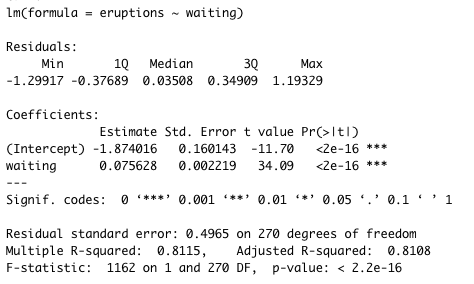
\includegraphics[scale=0.6]{images/regsum.png}
    \end{center}
    Let's pick this apart piece by piece.
\end{frame}

\begin{frame}{Regression Example}
    \begin{center}
        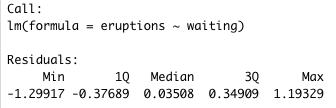
\includegraphics[scale=0.6]{images/regcall.png}
    \end{center}
    \begin{itemize}
        \item The first line shows the command used in \texttt{R} to run this regression model.
        \item The \texttt{Residuals} item shows a quartile-based summary of our residuals.
    \end{itemize}
\end{frame}

\begin{frame}{Regression Example}
    \begin{center}
        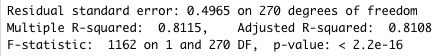
\includegraphics[scale=0.6]{images/regfstat.png}
    \end{center}
    The \texttt{F-statistic} and \texttt{p-value} give information about the model overall. 
    \begin{itemize}
        \item These are based on an F-distribution.
        \item The null hypothesis is that all of our model parameters are 0 (the model gives us no good info).
        \item Since p-value$ < 2.2\times10^{-16} < \alpha = 0.05$, at least one of the parameters is nonzero (the model is useful).
    \end{itemize}
\end{frame}

\begin{frame}{Regression Example}
    \begin{center}
        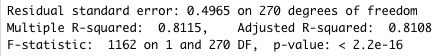
\includegraphics[scale=0.6]{images/regfstat.png}
    \end{center}
    \begin{itemize}
        \item \texttt{Multiple R-squared} is our squared correlation coefficient $R^2$. 
        \item Ignore the adjusted R-squared and residual standard error for now.
    \end{itemize}
\end{frame}

\begin{frame}{Regression Example}
    \begin{center}
        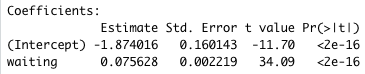
\includegraphics[scale=0.6]{images/regcoef.png}
    \end{center}
    Finally, the \texttt{Coefficients} section gives us several pieces of information:
    \begin{enumerate}
        \item \texttt{Estimate} shows the estimated parameters for each value.
        \item \texttt{Std. Error} gives the standard error for each parameter estimate.
        \item The \texttt{t values}s are the test statistics for each parameter estiamte.
        \item Finally, \texttt{Pr(>|t|)} are the p-values for each parameter estimate.
    \end{enumerate}
\end{frame}

\begin{frame}{Regression Example}
    The hypothesis test for each regression coefficient has hypotheses
    \begin{align*}
        H_0: \beta_i = 0 \\
        H_A: \beta_i \ne 0
    \end{align*}
    where $i=0$ for the intercept and $i=1$ for the slope.
\end{frame}

\begin{frame}{Regression Example}
    \begin{center}
        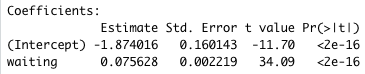
\includegraphics[scale=0.6]{images/regcoef.png}
    \end{center}
    \begin{enumerate}
        \item $p-value < 2\times10^{-16}$ for $b_0$ so we can conclude that the intercept is nonzero.
        \item $p-value < 2\times10^{-16}$ for $b_1$ so we conclude that the intercept is also nonzero.
        \item This means that the intercept and slope both provide useful information when predicting values of $y=\texttt{eruptions}$.
    \end{enumerate} 
\end{frame}